\documentclass{standalone}
\usepackage{tikz}
\usetikzlibrary{bayesnet}

% Provides the following node styles:

%     latent
%     obs
%     det
%     const
%     factor
%     plate
%     gate

% Provides the following commands (note that any of the arguments can be empty):

%     \factor [options] {name} {caption} {inputs} {outputs}
%     \plate [options] {name} {fitlist} {caption}
%     \gate [options] {name} {fitlist} {inputs}
%     \vgate {name} {fitlist-left} {caption-left} {fitlist-right} {caption-right} {inputs}
%     \hgate {name} {fitlist-top} {caption-top} {fitlist-bottom} {caption-bottom} {inputs}
%     \edge [options] {inputs} {outputs}
%     \factoredge [options] {inputs} {factors} {outputs}
\begin{document}
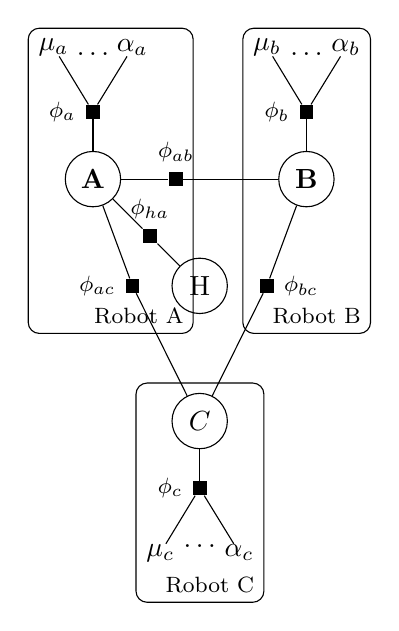
\begin{tikzpicture}

  % Define nodes

  % C
  \node[latent]          (c)   {$C$}; %
  % \factor[above=of y] {y-f} {left:$\mathcal{N}$} {} {} ; %
  
  % C hyperparameters
  \node[const, below=1.2 of c, xshift=-0.5cm] (mc) {$\mu_c$} ; %
  \node[const, below=1.2 of c]                (dc) {$\dots$} ; %
  \node[const, below=1.2 of c, xshift=+0.5cm] (ac) {$\alpha_c$} ; %

  % A and B
  \node[latent, above=of c]            (h) {H} ; % 
  \node[latent, above left=1.2 of h]  (a)   {$\mathbf{A}$}; %
  \node[latent, above right=1.2	 of h] (b)   {$\mathbf{B}$}; %

  % A hyperparameters
  \node[const, above=1.2 of a, xshift=-0.5cm] (ma) {$\mu_a$} ; %
  \node[const, above=1.2 of a]                (da) {$\dots$} ; %
  \node[const, above=1.2 of a, xshift=+0.5cm] (aa) {$\alpha_a$} ; %

  % B hyperparameters
  \node[const, above=1.2 of b, xshift=-0.5cm] (mb) {$\mu_b$} ; %
  \node[const, above=1.2 of b]                (db) {$\dots$} ; %
  \node[const, above=1.2 of b, xshift=+0.5cm] (ab) {$\alpha_b$} ; %

  % % Factors
  \factor[above=of a] {a-f} {left:$\mathcal{\phi}_a$} {} {}%{ma,aa} {a} ; %
  \factor[above=of b] {b-f} {left:$\mathcal{\phi}_b$} {} {}%{mb,ab} {b} ; %
  \factor[below=of c] {c-f} {left:$\mathcal{\phi}_c$} {} {}%{mc,ac} {c} ; %
  \factor[right=of a, xshift=+0.2cm] {a-f-b} {above:$\mathcal{\phi}_{ab}$} {} {} ; %
  \edge [-] {a,b} {a-f-b} ;
  \factor[right=of h] {c-f-b} {right:$\mathcal{\phi}_{bc}$} {} {} ; %
  \edge [-] {c,b} {c-f-b} ;
  \factor[left=of h] {c-f-a} {left:$\mathcal{\phi}_{ac}$} {} {} ; %
  \edge [-] {c,a} {c-f-a} ;
  \factor[above left=of h] {h-f-a} {above:$\mathcal{\phi}_{ha}$} {} {} ; %
  \edge [-] {h} {h-f-a};
  \edge [-] {h-f-a} {a};
  % all undirected
  \edge [-] {ma,aa} {a-f} 
  \edge [-] {a-f} {a}
  \edge [-] {mb,ab} {b-f} 
  \edge [-] {b-f} {b}
  \edge [-] {mc,ac} {c-f} 
  \edge [-] {c-f} {c}

  % blob or gate
  \plate {rob-a} {(ma)(da)(aa)(a)(c-f-a)(a-f-b)} {Robot A}
  \plate {rob-c} {(mb)(db)(ab)(b)(c-f-b)} {Robot B}
  \plate {rob-c} {(mc)(dc)(ac)(c)} {Robot C}


  % \fact

  % \factor[above right=of h] {h-f-b} {left:$\mathcal{\phi}_{hb}$} {} {} ; %
  % \edge {h} {h-f-b};
  % \edge {h-f-b} {b};
  % \factor[below=of h] {h-f-c} {above right, xshift=-0.2cm, yshift=-0.1cm:$\mathcal{\phi}_{hc}$} {} {} ; %
  % \edge {h} {h-f-c};
  % \edge {h-f-c} {c};

\end{tikzpicture}
\end{document}